\documentclass[12pt,a4paper]{article}

\usepackage[utf8]{inputenc}
\usepackage[T1]{fontenc}
\usepackage[brazilian]{babel}
\usepackage[a4paper,top=2.2cm,bottom=2.2cm,left=2.5cm,right=2.5cm]{geometry}
\usepackage{amsmath}
\usepackage{amssymb}
\usepackage{enumitem}
\usepackage{graphicx}
\usepackage{float}
\usepackage{caption}
\usepackage{microtype}
\usepackage{tabularx}
\usepackage{titlesec}
\usepackage[hidelinks]{hyperref}

\setlength{\parindent}{0pt}
\setlength{\parskip}{0.35em}
\captionsetup{aboveskip=2pt,belowskip=2pt}
\graphicspath{{prints/}}
\titlespacing*{\section}{0pt}{0.5em}{0.3em}
\titlespacing*{\subsection}{0pt}{0.45em}{0.2em}

\newcommand{\resposta}[1]{\textbf{Resposta:} #1}

\begin{document}

\begin{center}
    {\Large \textbf{TRABALHO T1 -- ELETR\^ONICA DE POT\^ENCIA}}\\[0.4em]
    {\normalsize Diodos e Tiristores}
\end{center}

\vspace{0.2em}

\begin{tabularx}{\linewidth}{@{}X c c c@{}}
\textbf{Acad\^emico(a):} Giuseph De Luka Giangareli &
\textbf{Semestre:} 7\textsuperscript{o} &
\textbf{Data:} 20/03/2026 &
\textbf{Nota:} \rule{1.8cm}{0.4pt}
\end{tabularx}

\vspace{0.25em}
{\small \textbf{Observa\c{c}\~ao:} os gr\'aficos deste trabalho foram gerados no GeoGebra, conforme solicitado no enunciado.}

\hrule
\vspace{0.5em}

\section*{Quest\~ao 1}

\noindent
\begin{minipage}[t]{0.66\linewidth}
\vspace{0pt}
\textbf{Enunciado:} Considere o circuito de malha \'unica com diodo ideal e resistor de \(10\,\Omega\), alimentado por \(v_s(t)=311\sin(377t)\,\text{V}\).
\end{minipage}
\hfill
\begin{minipage}[t]{0.30\linewidth}
\vspace{0pt}
    \centering
    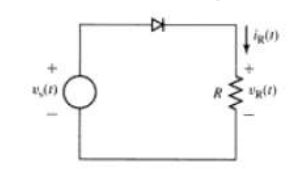
\includegraphics[width=0.92\linewidth,trim=10 6 10 6,clip]{grafico_Q1.png}
    
    {\small Circuito da Quest\~ao 1.}
\end{minipage}

\subsection*{(A) Esboce o gr\'afico do sinal de entrada}

\resposta{A tens\~ao de entrada \'e uma senoide completa, com valor de pico de \(311\,\text{V}\) e frequ\^encia angular de \(377\,\text{rad/s}\), o que corresponde a aproximadamente \(60\,\text{Hz}\).}

\begin{figure}[H]
    \centering
    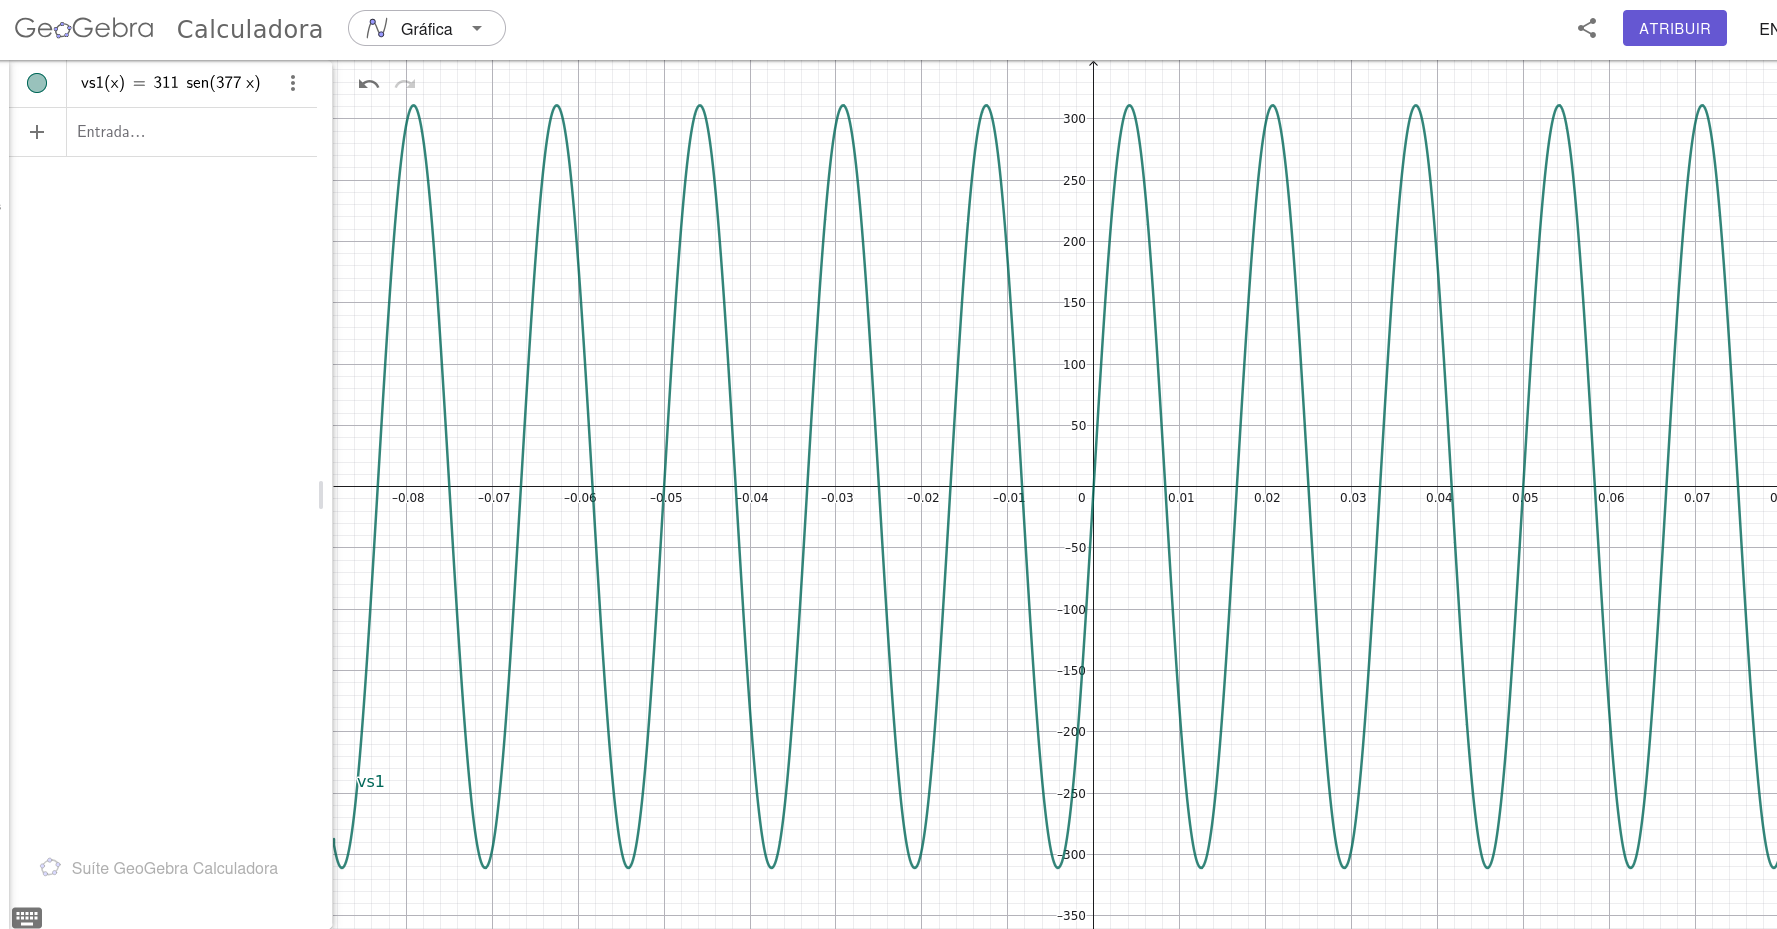
\includegraphics[width=\linewidth]{1a.png}
    \caption*{Gr\'afico de \(v_s(t)\) no GeoGebra.}
\end{figure}

\newpage

\subsection*{(B) Esboce o gr\'afico da tens\~ao \(v_R(t)\) no resistor}

\resposta{Como o diodo \'e ideal, ele conduz no semiciclo positivo e bloqueia no semiciclo negativo. Assim, a tens\~ao no resistor fica igual \`a tens\~ao da fonte somente quando \(v_s(t) \geq 0\), e vale zero no restante do tempo. Isso caracteriza uma retifica\c{c}\~ao de meia onda.}

\[
v_R(t)=
\begin{cases}
311\sin(377t), & \text{se } \sin(377t)\geq 0 \\[0.4em]
0, & \text{caso contr\'ario}
\end{cases}
\]

\begin{figure}[H]
    \centering
    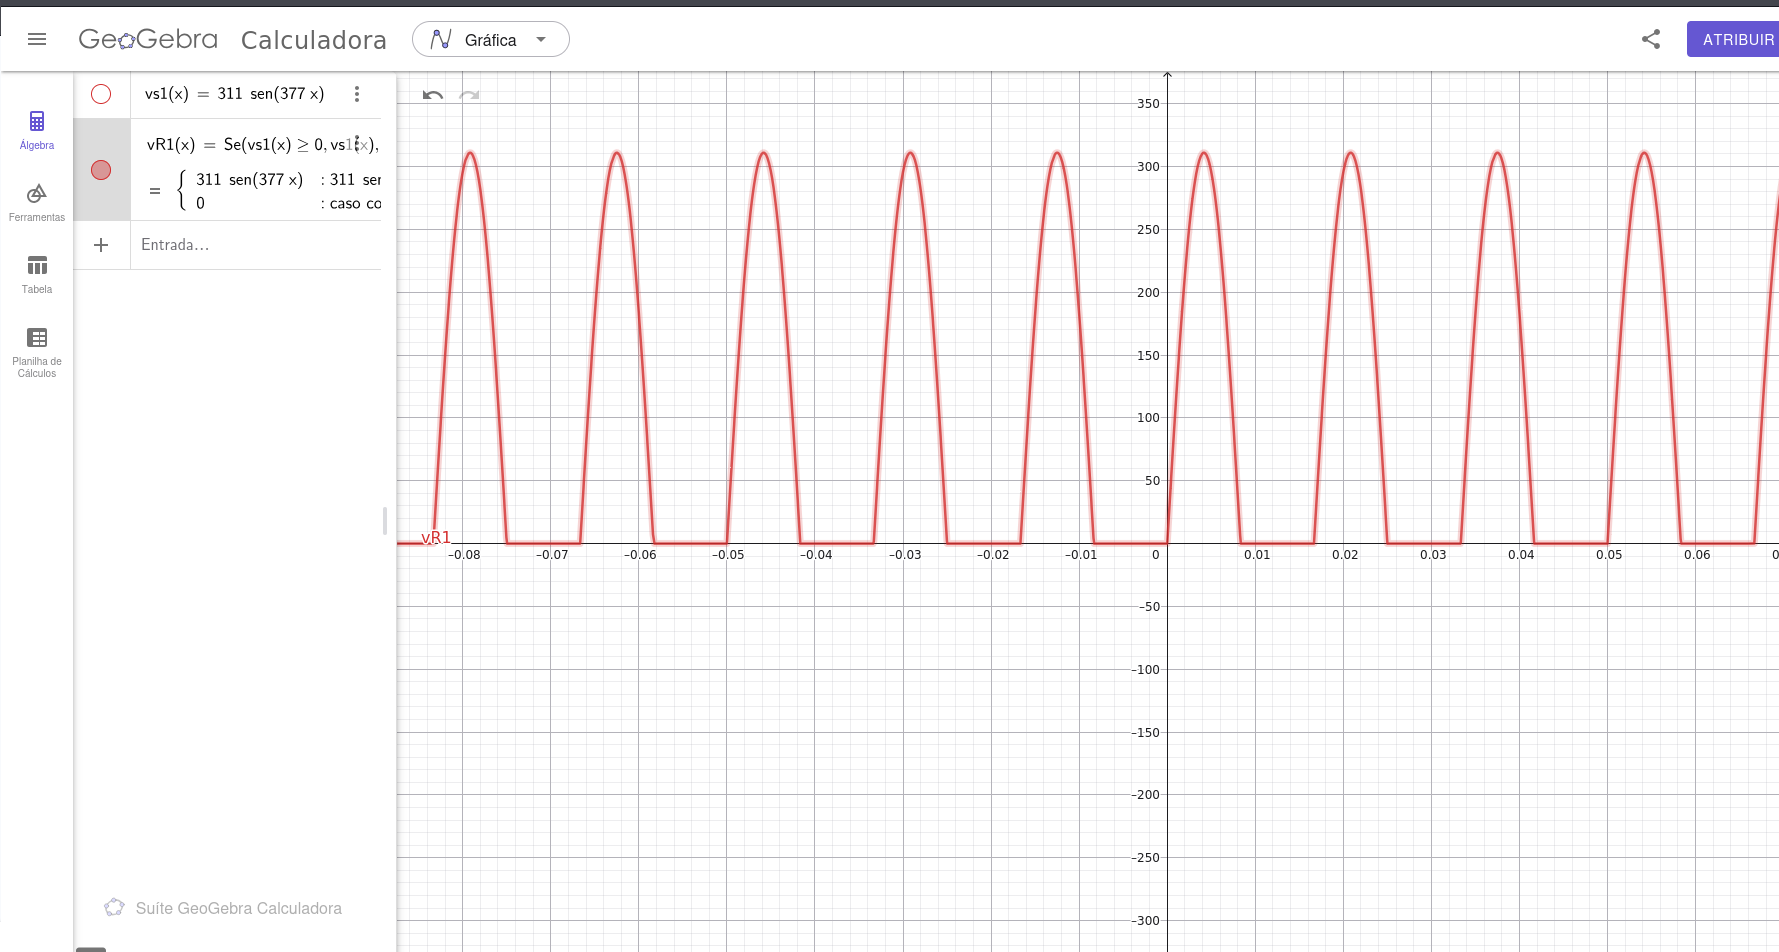
\includegraphics[width=\linewidth]{1b.png}
    \caption*{Gr\'afico de \(v_R(t)\) no resistor.}
\end{figure}

\newpage

\subsection*{(C) Esboce o gr\'afico da corrente \(i_R(t)\) no circuito}

\resposta{Pela primeira lei de Ohm, \(i_R(t)=\frac{v_R(t)}{R}\). Como \(R=10\,\Omega\), a corrente tem a mesma forma da tens\~ao no resistor, mudando apenas a amplitude. O valor de pico da corrente \'e \(311/10 = 31{,}1\,\text{A}\).}

\[
i_R(t)=
\begin{cases}
31{,}1\sin(377t), & \text{se } \sin(377t)\geq 0 \\[0.4em]
0, & \text{caso contr\'ario}
\end{cases}
\]

\begin{figure}[H]
    \centering
    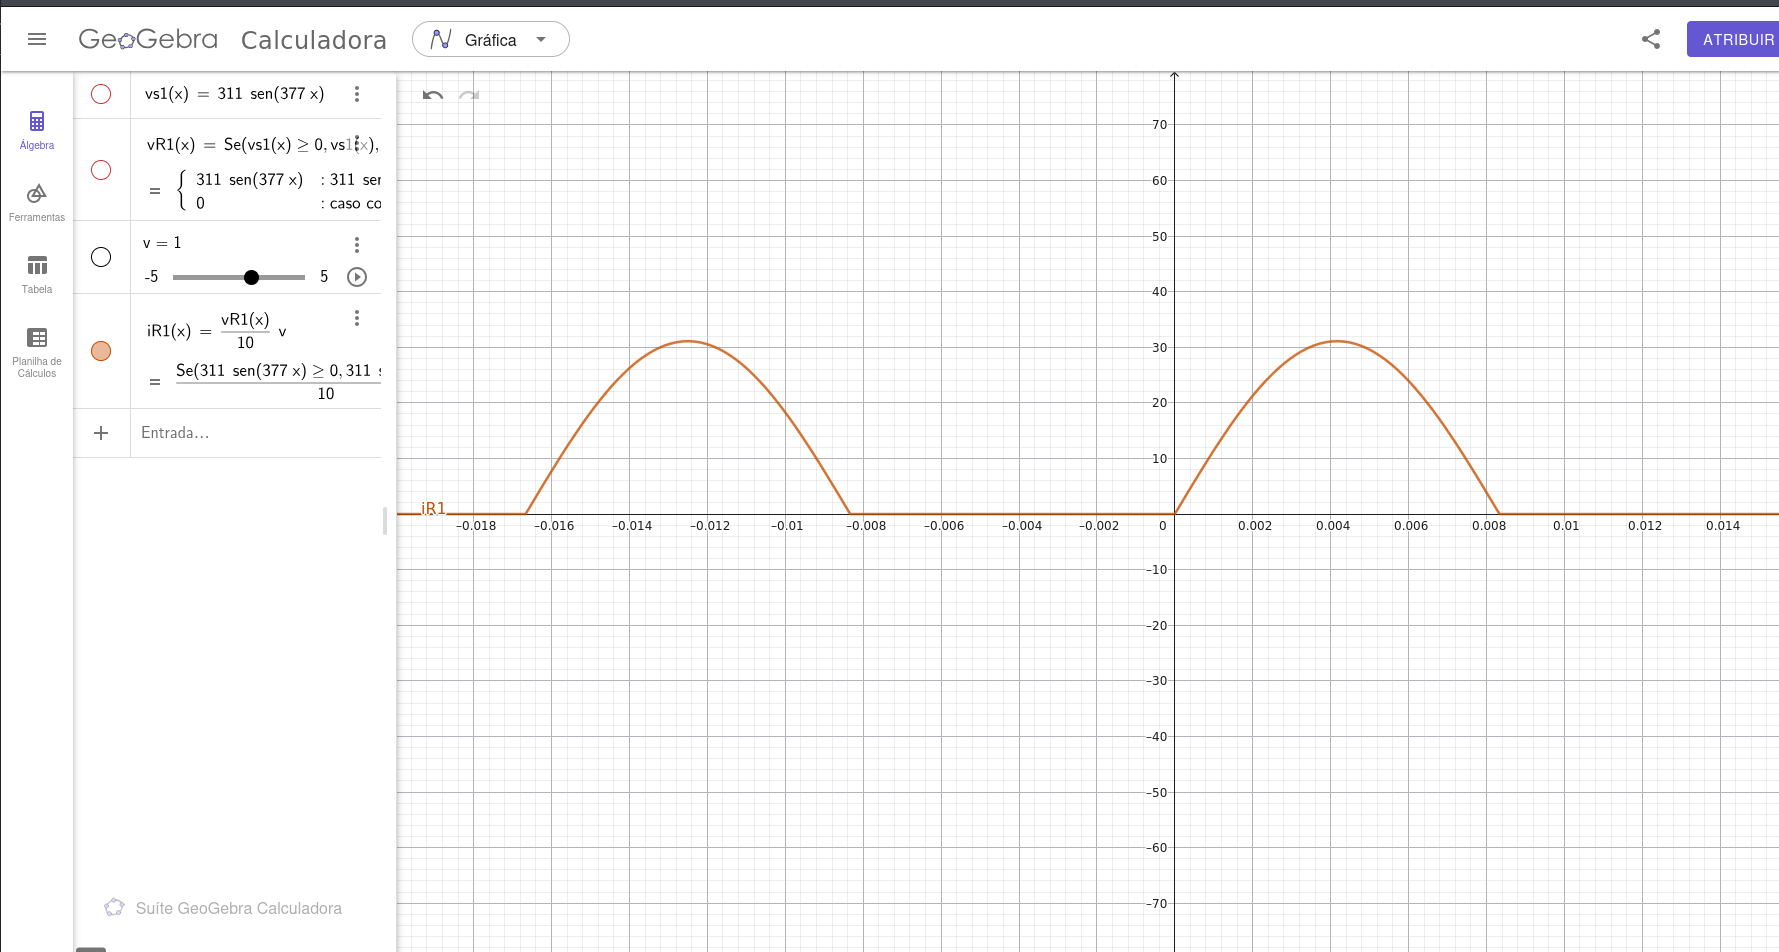
\includegraphics[width=\linewidth]{1c.png}
    \caption*{Gr\'afico de \(i_R(t)\) no resistor.}
\end{figure}

\newpage

\subsection*{(D) O que acontece se o resistor for trocado por outro com o dobro da resist\^encia?}

\resposta{Se o resistor passar de \(10\,\Omega\) para \(20\,\Omega\), a forma de onda da tens\~ao no resistor continua a mesma, porque o diodo e a fonte n\~ao mudaram. O que muda \'e a corrente, que cai pela metade. Nesse caso, o novo pico de corrente passa a ser \(311/20 = 15{,}55\,\text{A}\).
	
(Nao pediu grafico ,mas achei legal por !)
}
\begin{figure}[H]
    \centering
    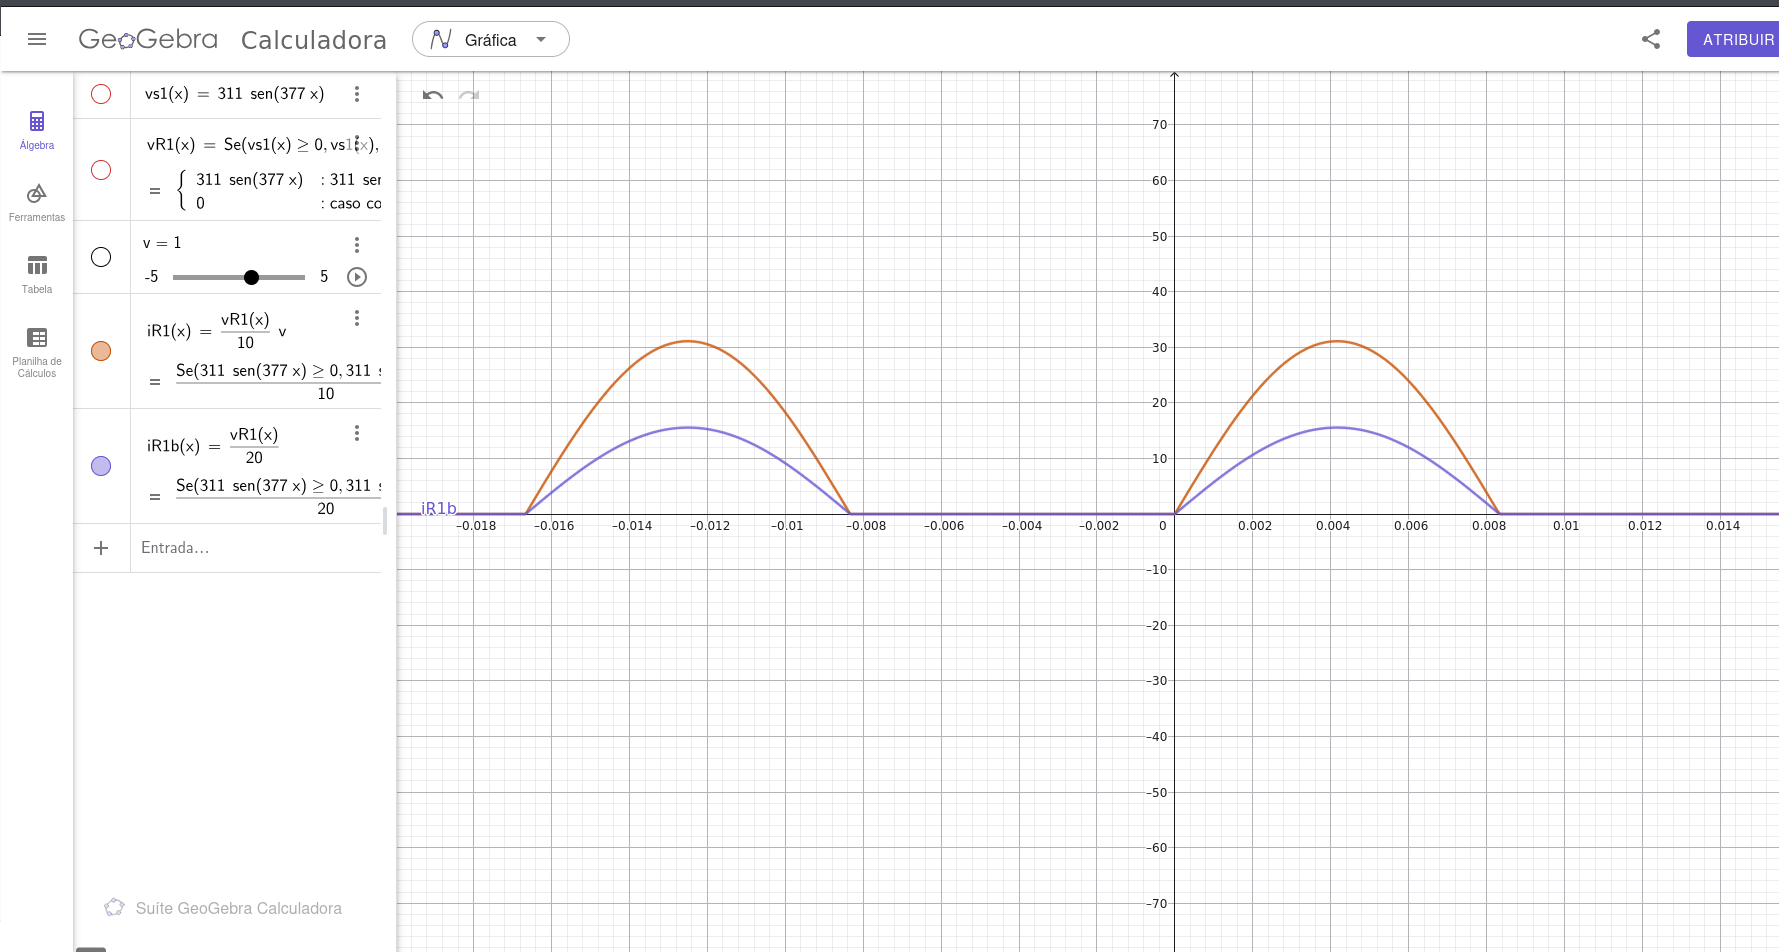
\includegraphics[width=\linewidth]{1d.png}
    \caption*{Compara\c{c}\~ao entre a corrente para \(10\,\Omega\) e para \(20\,\Omega\).}
\end{figure}

\subsection*{(E) O que acontece se a fonte de tens\~ao alternada for trocada por uma fonte CC?}

\resposta{Se a fonte CC polarizar o diodo diretamente, ele conduz continuamente. Nesse caso, a tens\~ao no resistor fica constante e a corrente tamb\'em fica constante, obedecendo \(i_R=\frac{V_{CC}}{10}\). Se a fonte CC polarizar o diodo inversamente, ele bloqueia a passagem de corrente e, portanto, \(v_R=0\) e \(i_R=0\).}

\vspace{0.4em}
\hrule
\vspace{0.5em}
\newpage

\section*{Quest\~ao 2}

\noindent
\begin{minipage}[t]{0.66\linewidth}
\vspace{0pt}
\textbf{Enunciado:} Considere o circuito com tiristor ideal e resistor de \(100\,\Omega\), alimentado por \(v_s(t)=179\sin(314t)\,\text{V}\), com disparos do tiristor em \(1{,}25\,\text{ms}\), \(11{,}25\,\text{ms}\) e \(21{,}25\,\text{ms}\).
\end{minipage}
\hfill
\begin{minipage}[t]{0.30\linewidth}
\vspace{0pt}
    \centering
    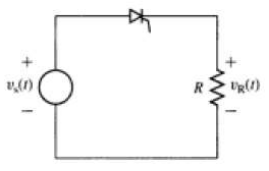
\includegraphics[width=0.92\linewidth,trim=10 6 10 6,clip]{grafico_Q2.png}
    
    {\small Circuito da Quest\~ao 2.}
\end{minipage}

\subsection*{(A) Esboce o gr\'afico do sinal de entrada}

\resposta{A tens\~ao de entrada \'e senoidal, com valor de pico de \(179\,\text{V}\) e frequ\^encia angular de \(314\,\text{rad/s}\), equivalente a aproximadamente \(50\,\text{Hz}\). Logo, o per\'iodo do sinal \'e \(T=20\,\text{ms}\) e cada semiciclo dura \(10\,\text{ms}\).}

\begin{figure}[H]
    \centering
    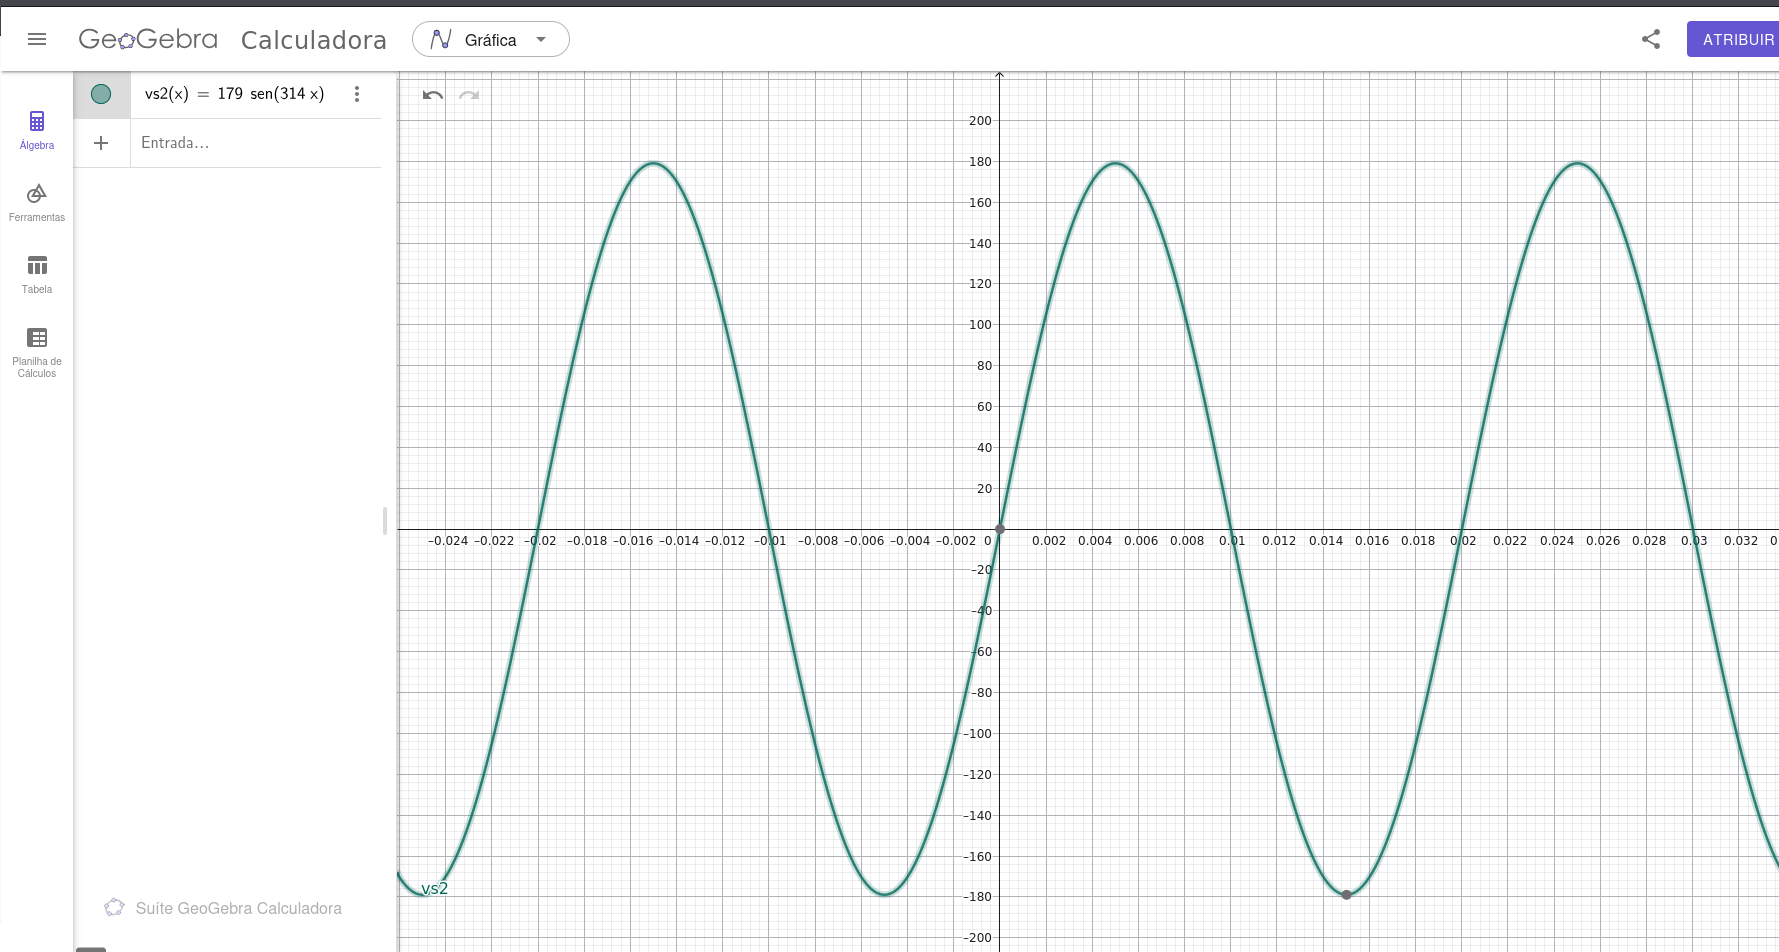
\includegraphics[width=\linewidth]{2a.png}
    \caption*{Gr\'afico de \(v_s(t)\) para a Quest\~ao 2.}
\end{figure}

\newpage

\subsection*{(B) Esboce o gr\'afico da tens\~ao \(v_R(t)\) no resistor}

\resposta{O tiristor s\'o conduz ap\'os receber o pulso de gatilho e desde que esteja diretamente polarizado. Como a carga \'e resistiva, depois do disparo ele permanece conduzindo at\'e o final do semiciclo positivo, quando a corrente zera naturalmente. Assim, de \(0\) a \(1{,}25\,\text{ms}\) a tens\~ao no resistor \'e zero; de \(1{,}25\,\text{ms}\) a \(10\,\text{ms}\), \(v_R(t)\) acompanha a fonte; de \(10\,\text{ms}\) a \(20\,\text{ms}\), a tens\~ao volta a zero. O disparo em \(11{,}25\,\text{ms}\) n\~ao liga o tiristor porque nesse intervalo ele est\'a reversamente polarizado.}

\[
v_R(t)=
\begin{cases}
179\sin(314t), & \text{durante os intervalos de condu\c{c}\~ao} \\[0.4em]
0, & \text{fora desses intervalos}
\end{cases}
\]

\begin{figure}[H]
    \centering
    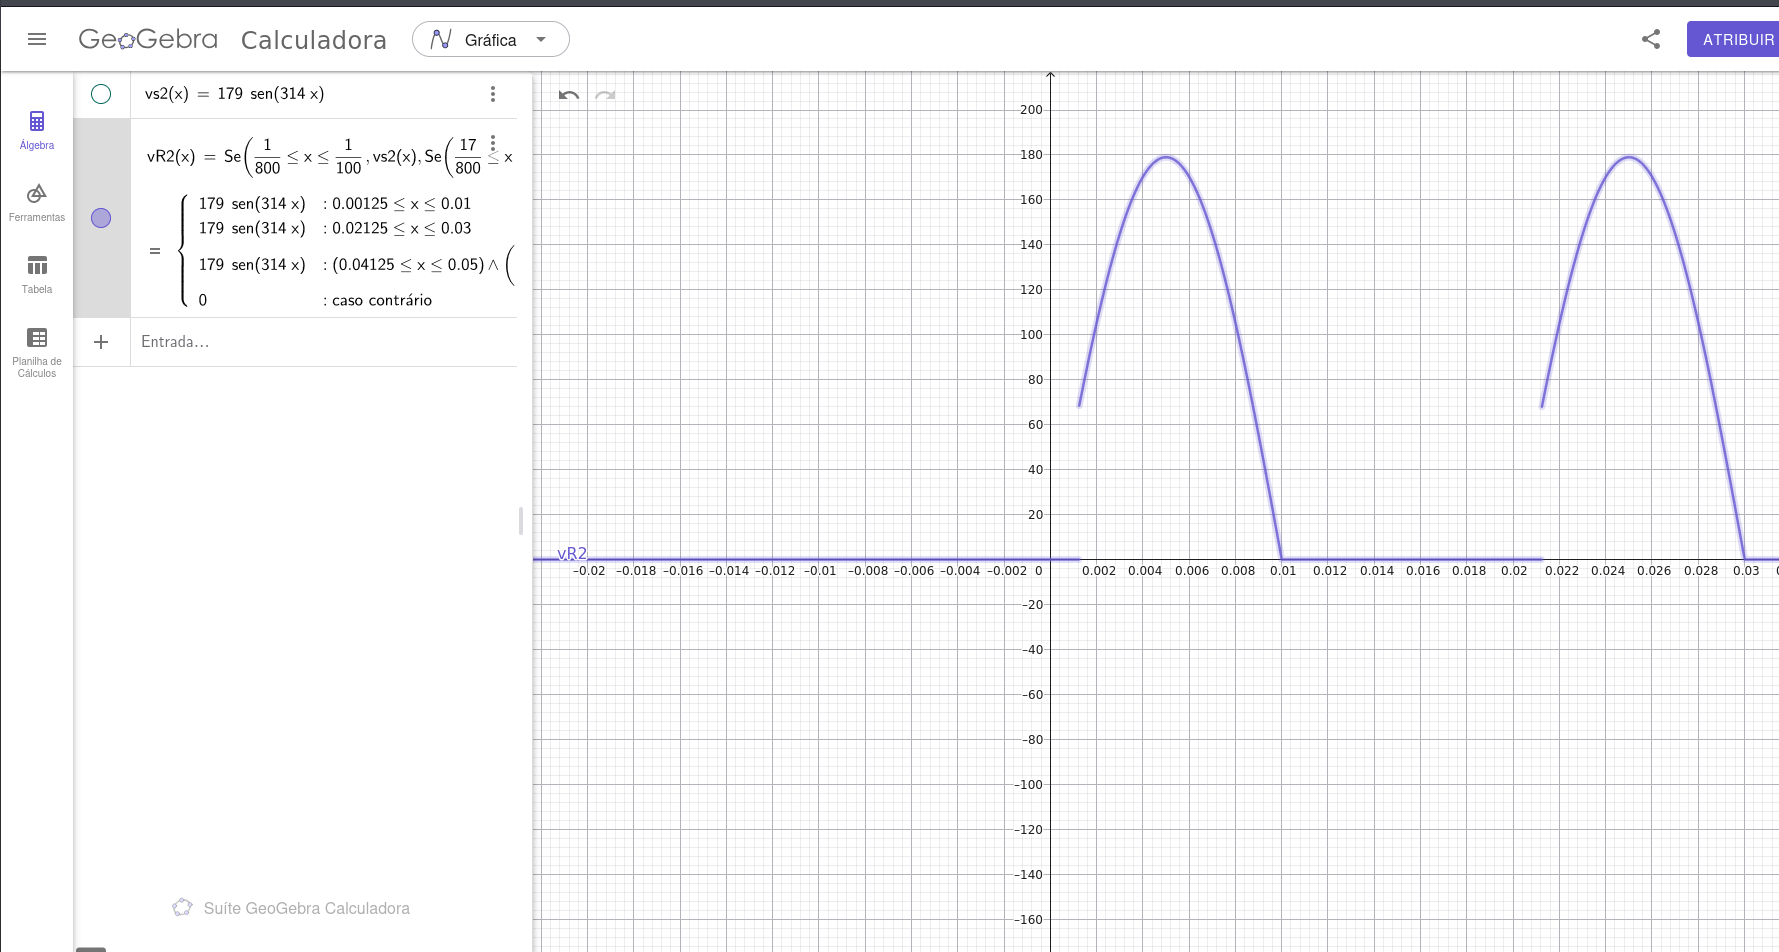
\includegraphics[width=\linewidth]{2b.png}
    \caption*{Gr\'afico de \(v_R(t)\) com disparo do SCR.}
\end{figure}

\subsection*{(C) O que acontece se o resistor for trocado por outro com o dobro da resist\^encia?}

\resposta{Se o resistor passar de \(100\,\Omega\) para \(200\,\Omega\), a forma de onda da tens\~ao no resistor n\~ao muda, porque os instantes de condu\c{c}\~ao continuam definidos pela fonte e pelo disparo do SCR. O que muda \'e a corrente, que cai pela metade. O pico da corrente passa de \(179/100 = 1{,}79\,\text{A}\) para \(179/200 = 0{,}895\,\text{A}\).}

\subsection*{(D) O que acontece se a fonte alternada for trocada por uma fonte CC?}

\resposta{Se a fonte CC estiver em polariza\c{c}\~ao direta, o SCR continua desligado at\'e receber um pulso no gatilho. Depois do disparo, no modelo ideal, ele entra em condu\c{c}\~ao e tende a permanecer ligado, porque em corrente cont\'inua a corrente n\~ao passa naturalmente por zero. Se a polaridade da fonte for inversa, o tiristor n\~ao conduz.}

\subsection*{(E) O que mudaria se a alimenta\c{c}\~ao fosse \(v_s(t)=5\sin(314t)\,\text{V}\)?}

\resposta{No modelo ideal, o comportamento geral continua o mesmo: o tiristor s\'o conduz ap\'os o disparo e apenas no semiciclo positivo em que estiver diretamente polarizado. A diferen\c{c}a \'e que a amplitude da tens\~ao no resistor fica bem menor. Com \(R=100\,\Omega\), a corrente de pico passa a ser \(5/100 = 0{,}05\,\text{A}\), ou seja, \(50\,\text{mA}\).}

\vfill
\hrule
\vspace{0.3em}
{\footnotesize
Eu usei o \LaTeX{} para escrever este trabalho. Caso voc\^e queira conferir o c\'odigo, ele est\'a dispon\'ivel no GitHub: \url{https://github.com/Giuseph66/TD_latex/tree/main/Trabalho_eletronica_potencia_T1}
}

\end{document}
